%%%%%%%%%%%%%%%%%%%%%%%%%%%%%%%%%%%%%%%%%%%%%%%%%%%%%%%%%%%%%%%%%%%%%%%%%%%%%%%%
%%  Eremeykin and Mirkin paper for "Avtomatika i Telemekhanika"               %%
%%%%%%%%%%%%%%%%%%%%%%%%%%%%%%%%%%%%%%%%%%%%%%%%%%%%%%%%%%%%%%%%%%%%%%%%%%%%%%%%

\documentclass[12pt]{a&t}
\usepackage{graphicx}

\begin{document}  %%%!!!

\year{2018}
\title{СОКРАЩЕНИЕ ВРЕМЕНИ ВЫЧИСЛЕНИЙ В АГЛОМЕРАТИВНОМ КЛАСТЕР-АНАЛИЗЕ ПЕРЕХОДОМ К ПОДВЫБОРКАМ}
\thanks{Тут пишут про финансовую поддержку.}

\authors{П.А.~ЕРЕМЕЙКИН, студент~НИУ~ВШЭ\\
Б.Г.~МИРКИН, док.~техн.~наук\\
(Национальный исследовательский университет\\ <<Высшая школа экономики>>, Москва)}

\maketitle

\begin{abstract}
Кластер-анализ находит широкое применение в различных областях деятельности. Наиболее популярный в настоящее время алгоритм кластеризации \mbox{k-means} обладает существенными недостатками, часть из которых удаётся успешно устранить благодаря современным исследованиям, предлагающим модернизации алгоритма. Одним из эффективных алгоритмов, предложенных в последнее время является \mbox{A-Ward$ _{p\beta} $}. Как любое новое решение, алгоритм \mbox{A-Ward$ _{p\beta} $} требует выработки рекомендаций по применению. Данная статья посвящена поиску способов определения параметров, задействованных в алгоритме. Ранее предлагаемые способы опираются на перебор всех возможных значений параметров в определённом интервале и требуют больших временных затрат. Для ускорения подбора параметров предлагается произвести переход к подвыборкам, существенно меньшего размера чем исходные данные и производить перебор для подвыборок. Авторы статьи предлагают рассмотреть различные способы формирования подвыборок и оценить эффективность этих способов с точки зрения затрачиваемого времени и качества результирующего разбиения.
%\begin{enumerate}
%	\item Написать аннотацию
%	\item Проверить ссылки на литературу и добавить в библиографию недостающие
%\end{enumerate}
\end{abstract}


\section{Введение}

Методы кластеризации широко применяются для выявления структуры данных и поиска характерных групп объектов. По принадлежности заданного нового объекта к определённому кластеру можно сделать предположения о ключевых свойствах этого объекта. В общем случае под кластеризацией понимают  поиск в заданном множестве  непересекающихся однородных подмножеств, которые включают в себя подобные объекты \cite{Mirkin-Vvedenie-v-analiz-dannyh}.
 
Наиболее широко известный и часто применяемый метод кластеризации --- \mbox{k-means} \cite{K-Means-canonical}. Этот метод состоит в попеременной минимизации квадратичного критерия по двум типам переменных: центрам кластеров и принадлежности объектов кластеру. Критерии минимизации аналогичного вида выражают смысл некоторых популярных иерархических алгоритмов, например, Ward \cite{Ward-canonical} или Bisecting \mbox{K-Means}\cite{Mirkin-Clustering-A-Data-Recovery-Approach}.

Несмотря на популярность алгоритма \mbox{k-means}, он обладает существенными недостатками. Во-первых, для работы необходимо явно задать число кластеров. В практических приложениях подлинное число кластеров как правило неизвестно. Во-вторых, \mbox{k-means} требует правильной инициализации начального состояния, от которого существенным образом зависит результат. И, наконец, алгоритм чувствителен к шуму в данных, то есть он не предусматривает никакого механизма учёта возможных погрешностей, которые зачастую возникают в реальных данных, полученных при помощи измерений.

За свою богатую историю алгоритм \mbox{k-means} получил множество усовершенствований, модификаций и новых применений. В частности, существенным вкладом в развитие алгоритма стала работа \cite{Anomalous-Clustring}, в которой предложен так называемый метод аномальных кластеров. Метод аномальных кластеров позволяет рационально определить начальное состояние для алгоритма \mbox{k-means} путём поочерёдного выявления и исключения кластеров, наиболее удалённых от центра данных, называемых аномальными. 

Иерархические алгоритмы, основанные на \mbox{k-means}, в основном наследуют его недостатки, но привносят важное свойство: в ходе работы они выявляют дерево вложенности кластеров, которое может быть естественным образом использовано в некоторых приложениях. Например, такое дерево может отражать  филогенетическое родство при кластеризации биологических видов. Это интересное свойство побуждает исследователей искать пути устранения недостатков иерархических алгоритмов, использующих квадратичный критерий. 

Как показали результаты экспериментов, проведённых в работе \cite{Amorim-Makarenkov-Mirkin}, метод аномальных кластеров в большинстве случаев порождает избыточное число кластеров, поэтому его можно использовать как предварительный шаг для агломеративного алгоритма Ward. Алгоритм Ward исходит из представления о том что на начальном этапе всякий единичный объект выступает в роли отдельного кластера и на каждом шаге происходит объединение двух ближайших кластеров пока их общее число не достигнет заданного значения.  Несмотря на то, что Ward в каноническом виде не требует инициализации, применение описанного предварительного шага вызвано необходимостью повышения производительности. При большом количестве объектов, на первых итерациях алгоритма требуется выполнить большое число сравнений (квадратично зависящее от числа объектов), и следовательно, время работы алгоритма в этом случае недопустимо велико. Благодаря применению предварительной проработки кластерной структуры с помощью аномального анализа отпадает необходимость сравнивать большое число кластеров в которых содержится всего по одному или несколько объектов. 

Описанная выше модификация получила название \mbox{A-Ward}. В той же работе \cite{Amorim-Makarenkov-Mirkin} предложено дальнейшее усовершенствование алгоритма \mbox{A-Ward}, которое акцентирует внимание на обработке зашумлённых данных. Обобщённая версия алгоритма для произвольной степени Минковского $ p $ и с использованием весовых коэффициентов признаков $ w $, определяемых отдельно для каждого кластера, была названа \mbox{A-Ward$ _{p\beta} $}, где $ \beta $ обозначает степень весовых коэффициентов $ w $.

Численные эксперименты на синтетических и реальных данных показали высокую эффективность алгоритма \mbox{A-Ward$ _{p\beta} $} в том числе для случаев с большой зашумленностью признаков, поэтому алгоритм представляет интерес для применения в практических случаях. Тем не менее, ввод новых параметров $ p $ и $ \beta $ породил необходимость выработки методики для определения их значений. В статье \cite{SW-Based-Search} рассмотрен подход к определению $ p $ и $ \beta $ методом перебора, в котором критерием качества результата служит эмпирическая характеристика Silhouette Width (SW)\cite{SW-Canonical}. Такой подход поглощает преимущество в производительности, достигнутое введением предварительного шага аномального кластер-анализа, и требует больших временных затрат.

Специалистам по анализу данных хорошо известна идея, которая лежит в основе принципа кросс-валидации \cite{CrossValidation-canonical} и заключается в сохранении основных свойств выборки даже в случае исключения из неё некоторой части объектов. Та же идея предположительно может быть использована для определения рациональных значений $ p $ и $ \beta $ по подвыборкам. Таким образом, в данной статье будет экспериментально исследована возможность выбора параметров $ p $ и $ \beta $ для алгоритма \mbox{A-Ward$ _{p\beta} $} путём перехода к подвыборкам и с использованием характеристики SW в качестве критерия качества результата.

\section{Предлагаемое решение}
\subsection{Описание эксперимента} \label{sec:experiment-description}
Пусть задано множество $ Y $ из $ N $ объектов, каждый из которых обладает $ V $ признаками. Такое множество можно выразить в виде таблицы данных:
\begin{gather} \label{eq:data-table}
	Y= \begin{pmatrix} 
	y_{1} \\
	\cdots \\ 
	y_{N} 
	\end{pmatrix}
	= \begin{pmatrix} 
		y_{11} & \cdots  & y_{1V} \\ 
		\cdots & \cdots  & \cdots \\ 
		y_{N1} & \cdots  & y_{NV} 
	\end{pmatrix}
\end{gather}
Алгоритм \mbox{A-Ward$ _{p\beta} $} при заданных значениях параметров $ p $ и $ \beta $  позволяет получить кластерное разбиение $ S=\{C_1, \ldots, C_K\} $  этого множества. Получаемое кластерное разбиение состоит из заранее определённого числа $ K $ непересекающихся кластеров $ C_k $, объединение которых покрывает всё множество объектов $ Y $. Принцип работы и формальное описание алгоритма \mbox{A-Ward$ _{p\beta} $} приведены в разделе \ref{sec:a-ward-p-beta}.

Для произвольного множества $ Y $ до сих про не было сформулировано эффективной методики поиска параметров  $ p $ и $ \beta $. Как было отмечено во введении, в статье \cite{SW-Based-Search} был опробован способ выбора параметров путём многократного запуска алгоритма \mbox{A-Ward$ _{p\beta} $} при переборе значений параметров в диапазоне $ \lbrack 1,5 \rbrack $ с шагом 0.1. Указанный диапазон определён исходя из опыта применения алгоритма: с превышением значений параметров 5 не достигается существенного улучшения качества разбиения. Нижняя граница диапазона определена математическим смыслом параметров.  

Описанный способ потребует $ 41^2= 1681 $ запуск алгоритма, что чрезвычайно затратно с точки зрения времени. Поэтому была предложена идея для определения значений параметров по случайным подвыборкам. Из всего множества $ Y $ выбирается $ L $ подмножеств $ Y_l \subset Y $ с заданным числом элементов $ n \ll N $. По каждому подмножеству  $ Y_l $ оцениваются рациональные значения параметров $ p^*_l $ и $ \beta^*_l $. Усреднённые по $ l $ значения $ p^* = \overline{p^*_l} $ и $ \beta^* = \overline{\beta^*_l} $ принимаются в качестве рационального выбора для всего множества $ Y $. При правильном выборе соотношения между числом объектов в полной выборке $ N $, числом объектов в подвыборке $ n $, и числом подвыборок $ M $, как ожидается, можно получить результат кластеризации близкий к результату, полученному с помощью оценки по всей выборке $ N $, затратив при этом существенно меньшее время.

Для подтверждения вышеописанных предположений предлагается рассмотреть численный эксперимент на синтетических данных. Синтетическая генерация позволяет гибко изменять характеристики данных, например число признаков и количество кластеров, степень их взаимного смешивания, а также определять истинное разбиение. Для генерации данных применяется метод описанный в статье \cite{Kovaleva}. Подробно его принцип работы разобран в разделе \ref{sec:data-generation}. Сейчас стоит иметь ввиду, что результат работы данного генератора синтетических данных полностью определяется следующими пятью параметрами:
\begin{enumerate}
	\item
	Число объектов $ N $
	\item
	Число признаков $ V $
	\item
	Количество кластеров $ K $
	\item 
	Минимальное число объектов в кластере $ m $
	\item
	Степень взаимного смешивания кластеров $ a \in \lbrack0,1\rbrack $
\end{enumerate}

Данные сгенерированные по методике, описанной в \cite{Kovaleva} мы будем обозначать ключевым словом \texttt{kovaleva}, за которым через подчёркивание следуют обозначения размерности (например \mbox{$\mathtt{1000 \times 15 } $}), общего числа кластеров с префиксом \texttt{с}, минимального числа объектов в кластере с префиксом \texttt{m} и, наконец, степени взаимного смешивания с префиксом \texttt{a}. В таблице \ref{tab:datasets} приведены три типа данных которые будут использованы в ходе эксперимента с пояснениями в принятых обозначениях. Данные, сгенерированные по указанным значениям параметров, обладают важным свойством: они соответствуют трём случаям, взаимного отношения числа признаков и количества кластеров. В первом случае число кластеров меньше числа признаков, во втором случае примерно равно, а в третьем --- больше.

\begin{table}[h!]
	\centering
	\caption{Параметры данных} \label{tab:datasets}
	\begin{tabular}{ |l|c|c|c|c|c| }
					\hline Обозначение               & N & V & K & m & a\\ 
					\hline $\mathtt{kovaleva\_1000 \times 15\_c7\_m100\_a0.5}$ & 1000 & 15 & 7 & 100 & 0.5\\ 
					\hline $\mathtt{kovaleva\_1000 \times 15\_c12\_m60\_a0.5}$ & 1000 & 15 & 12 & 60 & 0.5\\ 
					\hline $\mathtt{kovaleva\_1000 \times 15\_c19\_m35\_a0.5}$ & 1000 & 15 & 19 & 35 & 0.5\\ 
					\hline
	\end{tabular}
\end{table}

В ходе эксперимента будет рассмотрены четыре схем формирования подвыборки (без учёта полной выборки как эталонного случая). Первые две схемы представляют собой однократный выбор соответственно по 100 и 200 объектов, два оставшиеся~--- пятикратное формирование подвыборок по 100 и 200 объектов с последующим усреднением результата. В таблице \ref{tab:subsampling} приведены все пять рассматриваемых схем. 

\begin{table}[h!]
	\centering
	\caption{Схемы формирования подвыборки} \label{tab:subsampling}
	\begin{tabular}{ |l|c|c| }
		\hline Схема формирования подвыборки & \begin{tabular}{@{}c@{}}Размер подвыборки \\ $ n $\end{tabular} & \begin{tabular}{@{}c@{}}Число подвыборок  \\ $ L $\end{tabular}\\ 
		\hline Полная выборка (1-1000) & 1000 & 1 \\ 
		\hline Однокрантый выбор по 100 (1-100) & 100 & 1 \\ 
		\hline Однокрантый выбор по 200 (1-200) & 200 & 1 \\ 
		\hline Пятикрантый выбор по 100 (5-100) & 100 & 5 \\ 
		\hline Пятикрантый выбор по 200 (5-200) & 200 & 5 \\ 		
		\hline
	\end{tabular}
\end{table}

При применении алгоритма \mbox{A-Ward$ _{p\beta} $} на реальных данных для оценки качества результата и выбора наилучших значений  $ p $, $ \beta $  нет возможности использовать подлинное разбиение, поэтому популярный индекс ARI \cite{ARI-canonical} не подходит для применения в роли целевой характеристики. В качестве замены этому индексу может быть использована эмпирическая величина Silhouette Width (SW)\cite{SW-Canonical}, хорошо зарекомендовавшая себя во многих приложениях \cite{SW1,SW2}. Интересно также установить насколько использование эмпирической величины SW ухудшает результат относительно результата, полученного с использованием подлинного разбиения и индекса ARI. Синтетическая генерация данных позволит применить индекс ARI для оценки разбиений, получаемых при различных значениях параметров $ p $, $ \beta $, относительно истинного разбиения. Способы вычисления характеристики SW и индекса ARI описаны в разделах \ref{sec:sw} и \ref{sec:ari} соответственно.

При заданной характеристике качества может возникнуть ситуация неоднозначности при которой максимум достигается для нескольких пар параметров  $ p $ и $ \beta $. Для разрешения этой неоднозначности в рамках эксперимента предлагается рассмотреть два подхода:
\begin{enumerate}
	\item
	Предпочтение отдаётся паре параметров $ p $, $ \beta $ для которой величина $ p^2+\beta^2 $ минимальна
	\item
	Пусть $ \{(p_t, \beta_t): t=1,\ldots,T\} $ --- множество пар параметров для которых достигается максимум выбранной характеристики качества (SW или ARI). Рассчитаем поэлементные средние значения $ \overline{p} = \dfrac{1}{T}\sum_{t=1}^{T}p_t,\:\overline{\beta} = \dfrac{1}{T}\sum_{t=1}^{T}\beta_t $. Наилучшим выбором признается та пара, для которой значение $ (p_t-\overline{p})^2 + (\beta_t-\overline{\beta})^2 $ минимально.
\end{enumerate}

Ниже приведена формулировка алгоритма подбора параметров $ p $, $ \beta $, используемого в эксперименте. Описанный алгоритм применяется для синтетических данных из таблицы \ref{tab:datasets} c использованием в общей сложности пяти схем формирования подвыборки согласно таблице \ref{tab:subsampling}. При этом рассматриваются две характеристики качества разбиения: эмпирическая SW и индекс ARI, основанный на известном истинном разбиении. Для разрешения неопределённости выбора максимума характеристики рассматриваются два подхода, описанных в списке выше.

\begin{algorithm}[(Подбор параметров $ p $, $ \beta $ с переходом к подвыборкам)] \label{alg:experiment}
	\
	\begin{enumlist}[.] 
		\item
		Из множества $ Y $ случайным образом выбрать $ L $ подмножеств $ Y_l \subset Y $ с заданным размером $ n $. Пересечение выбранных подмножеств допускается.
		
		\item
		Для всех значений параметров $ p=1,1.1,\ldots,5 $ и $ \beta=1,1.1,\ldots,5 $ выполнить алгоритм \mbox{A-Ward$ _{p\beta} $} применительно к каждому подмножеству  $ Y_l $ и получить результирующее разбиение $ S_l^{p\beta} $.
		
		\item
		По каждому полученному разбиению  $ S_l^{p\beta} $ рассчитать значение характеристики Silhouette Width (или ARI): $ SW_l^{p\beta} = SW(S_l^{p\beta}) $.
		
		\item
		Для каждого подмножества $ Y_l $ выбрать рациональные значения параметров $ p $ и $ \beta $, соответствующие максимальным значениям характеристики Silhouette Width (или ARI): $ (p^*_l,\beta^*_l)=\operatorname{arg\,max}\{SW_l^{p\beta}\} $. В случае, если максимум достигается для нескольких пар параметров, рассмотреть два возможных подхода разрешения неоднозначности. 
		
		\item Результатом работы алгоритма являются усреднённые по $ l $ значения параметров $ p^* = \overline{p^*_l} $ и $ \beta^* = \overline{\beta^*_l} $. 
		
	\end{enumlist}
\end{algorithm}

\subsection{Алгоритм \mbox{A-Ward$ _{p\beta} $}} \label{sec:a-ward-p-beta}

Описание алгоритма \mbox{A-Ward$ _{p\beta} $} следует начать с рассмотрения общего принципа работы иерархических алгоритмов. В отличие от неиерархических алгоритмов, которые формируют плоскую структуру кластеров, как, например, \mbox{k-means}, иерархические алгоритмы в качестве результата предоставляют дополнительную информацию относительно взаимосвязей между кластерами. Эта информация выражена в виде вложенной последовательности разбиений \cite{Amorim-Makarenkov-Mirkin} и графически может быть изображена с помощью дендрограммы. На каждом уровне дендрограммы определённый объект $ y_i \in Y$ принадлежит единственному кластеру $ C_k $. В то же время этот объект может принадлежать на других уровнях другим кластерам, которые образованы разбиением кластера $ C_k $ или слиянием с другими кластерами. 

Различают два вида иерархический  алгоритмов: агломеративные (объединяющие) и дивизивные (разделяющие). Агломеративные алгоритмы работают по принципу ``снизу верх''. На начальном этапе работы таких алгоритмов каждый единичный объект выступает в роли кластера. Во время работы происходит попарное объединение кластеров до тех пор, пока не будет достигнуто заданное число кластеров. Дивизивные алгоритмы в противоположность агломеративным действуют ``сверху вниз''.

Алгоритм Ward, усовершенствованием которого является алгоритм \mbox{A-Ward$ _{p\beta} $}, относится к агломеративным. На каждой итерации происходит слияние ближайших кластеров, таким образом чтобы внутрикластерная дисперсия была минимальной. Исходя из принципа работы алгоритма Ward видно, что на начальных этапах происходит сравнение большого числа кластеров, примерно равного числу объектов, что требует продолжительного время вычисления. Решением этой проблемы является метод аномальных кластеров, выполняющий роль инициализации. Инициализация осуществляется в две стадии: на первой выявляются аномальные кластеры (алгоритм \ref{alg:anomalous-p-beta}), а на второй происходит их стабилизация (алгоритм \ref{alg:imwk-means}). Ниже описан алгоритм взвешенной аномальной кластеризации для общего случая степени Минковского $ p $ и степени весовых коэффициентов $ \beta $.



\begin{algorithm}[(Инициализация аномальными кластерами)] \label{alg:anomalous-p-beta}
	\
	\begin{enumlist}[.] 
		
		\item \textit{Инициализация.} Задаться значениями параметров $ p $ и $ \beta $. Глобальный центр данных $ c_Y $ вычислить как покомпонентный центр Минковского по всем объектам \mbox{$ y_i \in Y $.}
		
		\item \label{itm:anomalous-p-beta-tent-centroid} \textit{Текущий центр.} Задать пустой аномальный кластер $ C_t = \varnothing $. Веса равномерно распределить по всем признакам $ w_{kv} = 1/V $ при $ k=1,2 $ и $ v=1,\ldots,V $. Текущий центр аномального кластера $ c_t $ выбрать как объект, наиболее удалённый от глобального центра $ c_Y $. Расстояние между объектом $ y_i $ и центром произвольного кластера $ c_k $ вычисляется по формуле:
		\begin{gather} \label{eq:obj-to-centroid-distance}
			d_{p\beta}(y_i,c_k)=\sum_{v=1}^{V}w^\beta_{kv}|y_{iv}-c_{kv}|^p
		\end{gather}
		
		\item \textit{Формирование аномального кластера.} В аномальный кластер добавить объекты, которые расположены ближе к текущему центру аномального кластера $ c_t $, чем к глобальному центру $ c_Y $ согласно расстоянию, определяемому формулой \ref{eq:obj-to-centroid-distance}. Если изменений в разбиении нет, прейти к шагу \ref{itm:anomalous-p-beta-save}.
		
		\item \textit{Обновление текущего центра.} Вычислить текущий центр аномального кластера $ c_t $ как покомпонентный центр Минковского по всем объектам в аномальном кластере $ y_i \in C_t $.
		
		\item \textit{Обновление весов.} Вычислить веса признаков по следующей формуле:
		\begin{gather} \label{eq:weights}
			w_{kv}=\dfrac{1}{\sum_{u=1}^{V} \left ( \dfrac{D_{kv}}{D_{ku}} \right )^{\frac{1}{\beta-1}}},
		\end{gather}
		\begin{tabular}{llll}
			где & $D_{kv}=\sum_{i\in C_k}^{}|y_{iv}-c_{kv}|^\beta$ & {---} & разброс признака $ v $ в кластере $ C_k $ \\
		\end{tabular}
		
		\item \label{itm:anomalous-p-beta-save} \textit{Сохранение параметров.} Включить текущий центр аномального кластера $ c_t $ в список центров $ \mathtt{c\_list} $, а веса $ w $ в список весов $ \mathtt{w\_list} $.
		
		\item \textit{Исключение аномального кластера.} Исключить из $ Y $ все объекты $ y_i \in C_t $. Если $ Y \neq \varnothing $, перейти к шагу \ref{itm:anomalous-p-beta-tent-centroid}.			
		
		\item \textit{ Результат.} Результатом работы алгоритма является разбиение S, а также списки центров кластеров $ \mathtt{c\_list} $ и весов $ \mathtt{w\_list} $.
	\end{enumlist}
\end{algorithm}

Характерная особенность структуры данных, генерируемой алгоритмом \ref{alg:anomalous-p-beta} состоит в том, что, во-первых, число получаемых кластеров всегда больше, чем их действительное количество, а во-вторых, что эта структура сгущается ближе к центру данных. Для смягчения второй особенности применяется вариация \mbox{k-means}, которая использует те же параметры степени Минковского $ p $ и степени весовых коэффициентов $ \beta $, а также начальное состояние, порождённое алгоритмом аномальной инициализации. Эта вариация получила название \mbox{$ imwk$-means$_{p\beta} $} и описана ниже.

\begin{algorithm}[(\mbox{$ imwk$-means$_{p\beta} $})] \label{alg:imwk-means}
	\
	\begin{enumlist}[.] 
		
		\item \textit{Инициализация.} Установить текущее разбиение пустым $ S=\varnothing $, а число кластеров $ K $ равным длине списка $ \mathtt{c\_list} $, который был получен при аномальной инициализации. 
		
		\item \label{itm:imwl-means-assignment}\textit{Формирование кластеров.} Каждый объект $ y_i \in Y $ поместить в кластер, центр которого $ c_k $ находится ближе всего к этому объекту. Близость объекта к центру кластера определяется  по формуле \ref{eq:obj-to-centroid-distance}. Если нет изменений в разбиении $  S $, перейти к шагу \ref{itm:imwl-means-result}.
		
		\item \textit{Обновление центров.} Вычислить новые координаты центра $ c_k $ каждого кластера $ C_k $ как покомпонентный центр Минковского всех объектов этого кластера $ y_i \in C_k $.
		
		\item \textit{Обновление весов.} Вычислить новые веса $ w_{kv} $ по формуле \ref{eq:weights} для $ k=1,\ldots,K $ и $ v=1,\ldots,V $. Перейти к шагу \ref{itm:imwl-means-assignment}
		
		\item \label{itm:imwl-means-result} \textit{ Результат.} Результатом работы алгоритма является разбиение S, а также списки центров кластеров $ \mathtt{c\_list} $ и весов $ \mathtt{w\_list} $.
	\end{enumlist}
\end{algorithm}

Итоговое разбиение строится агломеративным методом, обеспечивая заданное число кластеров. Модификация алгоритма Word с учетом весов признаков и для произвольной степени Минковского описана ниже.


\begin{algorithm}[(\mbox{A-Ward$ _{p\beta} $})] \label{alg:a-ward-p-beta}
	\
	\begin{enumlist}[.] 
		\item \textit{Инициализация.} Параметры $ p $ и $ \beta $ остаются неизменными, которые были определены для \mbox{$ imwk$-means$_{p\beta} $}. Начальное состояние соответствует конечному для \mbox{$ imwk$-means$_{p\beta} $}: исходный список центров кластеров $ \mathtt{c\_list} $ и весов $ \mathtt{w\_list} $ является результатом работы предыдущего этапа.
		
		\item \label{itm:a-ward-p-beta-merge} \textit{Объединение кластеров.} Выбрать два ближайших кластера $ C_a,\:C_b \in S$ и объединить их в новый $ C_{ab} $. Близость кластеров определяется по следующей формуле: 
		\begin{gather} \label{eq:ward-p-beta-distance}
		d_{Ward}(C_a,C_b)=\dfrac{N_aN_b}{N_a+N_b}\sum_{v=1}^{V}\left ( \frac{w_{av}+w_{bv}}{2} \right )^\beta |c_{av}-c_{bv}|^p,
		\end{gather}
		
		\begin{tabular}{llll}
			где & $ N_a,\:N_b $ & {---} & количество объектов в кластерах $ C_a $ и $ C_b $ соответственно \\
			& $ V $ & {---} & число признаков у каждого объекта $ y_i \in Y $ \\
			& $w_{av},\:w_{bv} $ & {---} & веса $ v $-го признака в кластере $ C_a $ и $ C_b $ соответственно \\
			& $ c_{av},\:c_{bv} $ & {---} & $ v $-ая координата центров кластеров $ C_a $ и $ C_b $ соответственно 
		\end{tabular}
		
		\item \textit{Обновление центра.} Вычислить новое значение центра $ C_{ab} $ как покомпонентный центр Минковского по всем объектам $ y_i \in C_{ab} $.
		
		\item \textit{Обновление весов.} Вычислить новые веса $ w_{kv} $ по формуле \ref{eq:weights} для $ k=1,\ldots,K $ и $ v=1,\ldots,V $.
		
		\item \textit{Условие остановки.} Уменьшить текущее число кластеров на единицу. Если текуще число кластеров все ещё больше единицы или требуемого числа кластеров, прейти к шагу \ref{itm:a-ward-p-beta-merge} .
			
	\end{enumlist}
\end{algorithm}


Алгоритм \mbox{A-Ward$ _{p\beta} $} хорошо зарекомендовал себя при тестах как на синтетических, так и на реальных данных. Особый интерес представляют возможности алгоритма при обработки зашумленных данных. Благодаря описанным нововведениям алгоритмом учитывается различные признаки с учётом их дисперсии в каждом кластере. 

\subsection{Генератор данных}\label{sec:data-generation}
Для генерации данных используется простой, но удобный подход, описанный в работе \cite{Kovaleva}. Используя единственный параметр, предложенный генератор позволяет регулировать разброс объектов внутри кластера и одновременно взаимное смешивание кластеров.

Структура получаемых данных представляют собой заданное количество гауссовых кластеров $ K $, сформированных при фиксированном общем числе объектов $ N $ и признаков $ V $ и определённом минимальном количестве объектов в каждом кластере $ m $. Остаток объектов $ \delta = N - K\cdot m $ распределяется случайно и равновероятно по всем кластерам. 

Кластеры порождается независимо гауссовым распределением. Центры кластеров генерируется как случайный $ V $-мерный вектор с равной вероятностью внутри гиперкуба $ [-a,a]^V $. При этом параметр $ a \in [0,1] $ отвечает за степень взаимного смешивания кластеров: чем больше значение параметра, тем сложнее разделить соседние кластеры. Ковариационная матрица кластеров генерируется со случайными диагональными элементами, значения которых равномерно распределены в диапазоне $ [0.025,\:0.05] $.

\subsection{Характеристика разбиения Silhouette Width}\label{sec:sw}
Эмпирическая характеристика Silhouette Width (SW) \cite{SW-Canonical} позволяет оценить качество разбиения непосредственно, не опираясь на известное эталонное разбиение, поэтому она хорошо подходит для поиска параметров алгоритма \mbox{A-Ward$ _{p\beta} $} на реальных данных. Для воспроизведения этой ситуации SW будет использована в эксперименте. 

Значение характеристики для разбиения $ S $ определяется как среднее значение SW для всех объектов $ y_i \in Y $. Silhouette Width для одного объекта рассчитывается по следующей формуле:

\begin{gather} \label{eq:sw}
SW(y_i) = \dfrac{b(y_i)-a(y_i)}{max\{a(y_i),b(y_i))\}}
\end{gather}

\begin{tabular}{llll}
	где & $ a(y_i) $ & {---} & среднее расстояние между объектом $ y_i \in C_k $ и всеми объектами, \\
	& & &	принадлежащими тому же кластеру $ C_k $, что и $ y_i $, \\
	& $ b(y_i) $ & {---} & наименьшее среднее расстояние между объектом $ y_i \in C_k $ и \\
	& & &  объектами, которые принадлежат другим кластерам. \\
\end{tabular}

Значения характеристики SW лежат в промежутке от -1 до 1. Разбиения, для которых характеристика SW ближе к 1 предпочтительнее тех, у которых SW меньше.

\subsection{Индекс ARI}\label{sec:ari}
Индекс ARI (Adjusted Rand Index) \cite{ARI-canonical} является популярным способом сравнения эталонного и заданного разбиения. В условиях проводимого эксперимента используются синтетические данные, для которых известно истинное разбиение, поэтому для оценки эффективности применения эмпирической характеристики SW можно задействовать ARI. Формула для вычисления индекса записывается следующим образом:

\begin{gather} \label{eq:ari}
ARI = \dfrac{\sum_{ij}\binom{n_{ij}}{2}-\left [ \sum_{i}\binom{a_{i}}{2}\sum_{j}\binom{b_{j}}{2} \right ]/\binom{n}{2}}{\dfrac{1}{2} \left [ \sum_i \binom{a_i}{2} + \sum_j \binom{b_j}{2} \right ] - \left [ \sum_i \binom{a_i}{2} \sum_j \binom{b_j}{2} \right ]/ \binom{n}{2}}
\end{gather}
 

\begin{tabular}{llll}
	где & $ n_{ij} = |C_i \cap C_j| $ & {---} & число объектов, входящий одновременно в $ i $-ый \\  
	& & &кластер в первом разбиении и в $ j $-ый --- во втором. \\
	& $ a_{i} = \sum_{j=1}^{K} |C_i \cap C_j| $ & {---} & число объектов, ходящих в $ i $-ый кластер в первом \\
	& & &разбиении\\
	& $ b_{j} = \sum_{i=1}^{K} |C_i \cap C_j| $ & {---} & число объектов, ходящих в $ j $-ый кластер во втором\\		
	& & & разбиении\\
\end{tabular}

Как и характеристика SW, индекс ARI принимает значения от -1 до 1. ARI достигает 1 только в том случае, если два разбиения совпадают.

%\section{Организация эксперимента}

\section{Результаты эксперимента}
Результаты эксперимента приведены на рисунке \ref{fig:plots}, который состоит из трёх строк и трёх столбцов. Первая строка содержит диаграммы, на которых закрашенными столбцами изображено среднее значение индекса ARI, вычисленного относительно разбиения, полученного как результат работы \mbox{A-Ward$ _{p\beta} $}, с параметрами $ p $ и $ \beta $, определёнными по алгоритму \ref{alg:experiment} с критерием качества SW. Вторая строка отличается от первой тем, что в роли критерия качества вместо SW был использован индекс ARI относительно истинного разбиения. В третьей строке изображены диаграммы для суммарного времени работы \mbox{A-Ward$ _{p\beta} $} на заданных подвыбокрах без учёта вычисления критериев качества. Эксперименты проводились на ПК с процессором  Intel\textsuperscript{\textregistered} Core\textsuperscript{\texttrademark}2 Quad Q9550, работающем на частоте 2.83 ГГц и с объёмом оперативной памяти 4 Гб.

 Столбцы на рисунке \ref{fig:plots} соответствуют трём вариантам количества кластеров в сгенерированных данных: 7, 12 или 19. Тонкими линиями показаны среднеквадратичное отклонения, вычисленные по 10 экспериментам. Цвет столбца определяет один из двух анализируемых подходов разрешения неопределённости, которые описаны в разделе \ref{sec:experiment-description}. Красный соответствует первому подходу, а синий --- второму.
   
\begin{figure}[!h]
	\begin{center}
		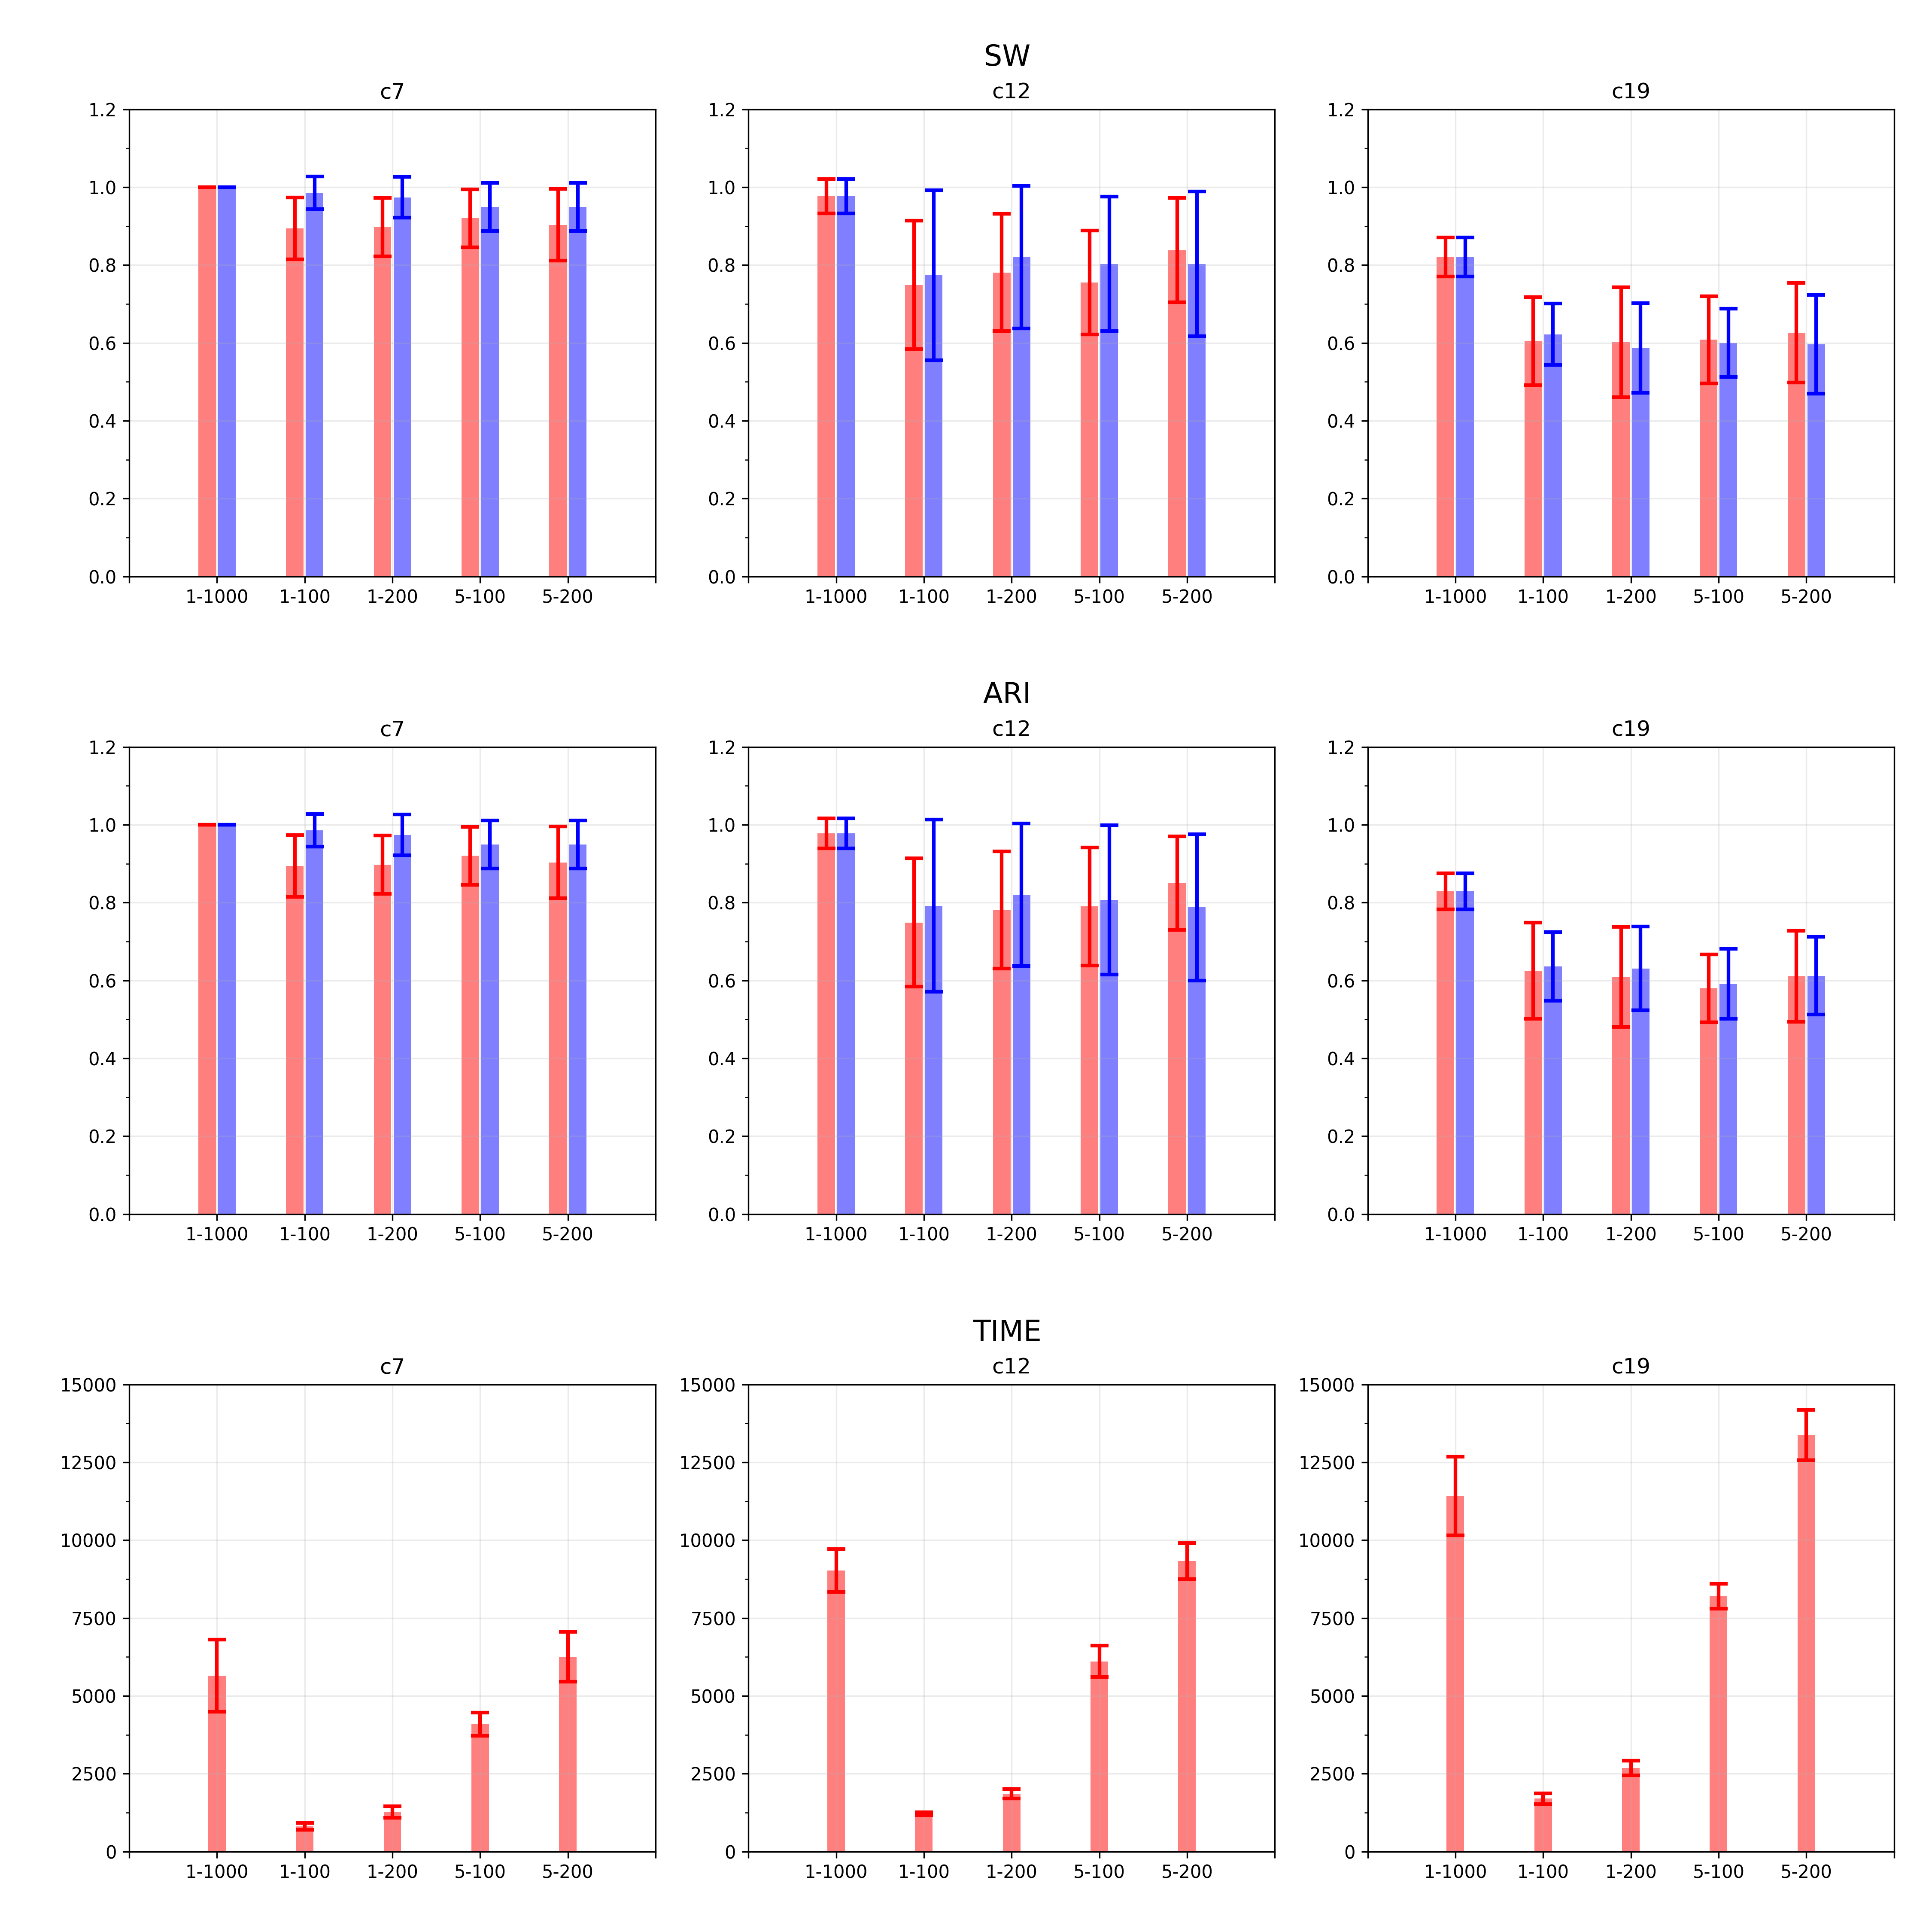
\includegraphics[width=\textwidth]{imgs/bars.png} 
%		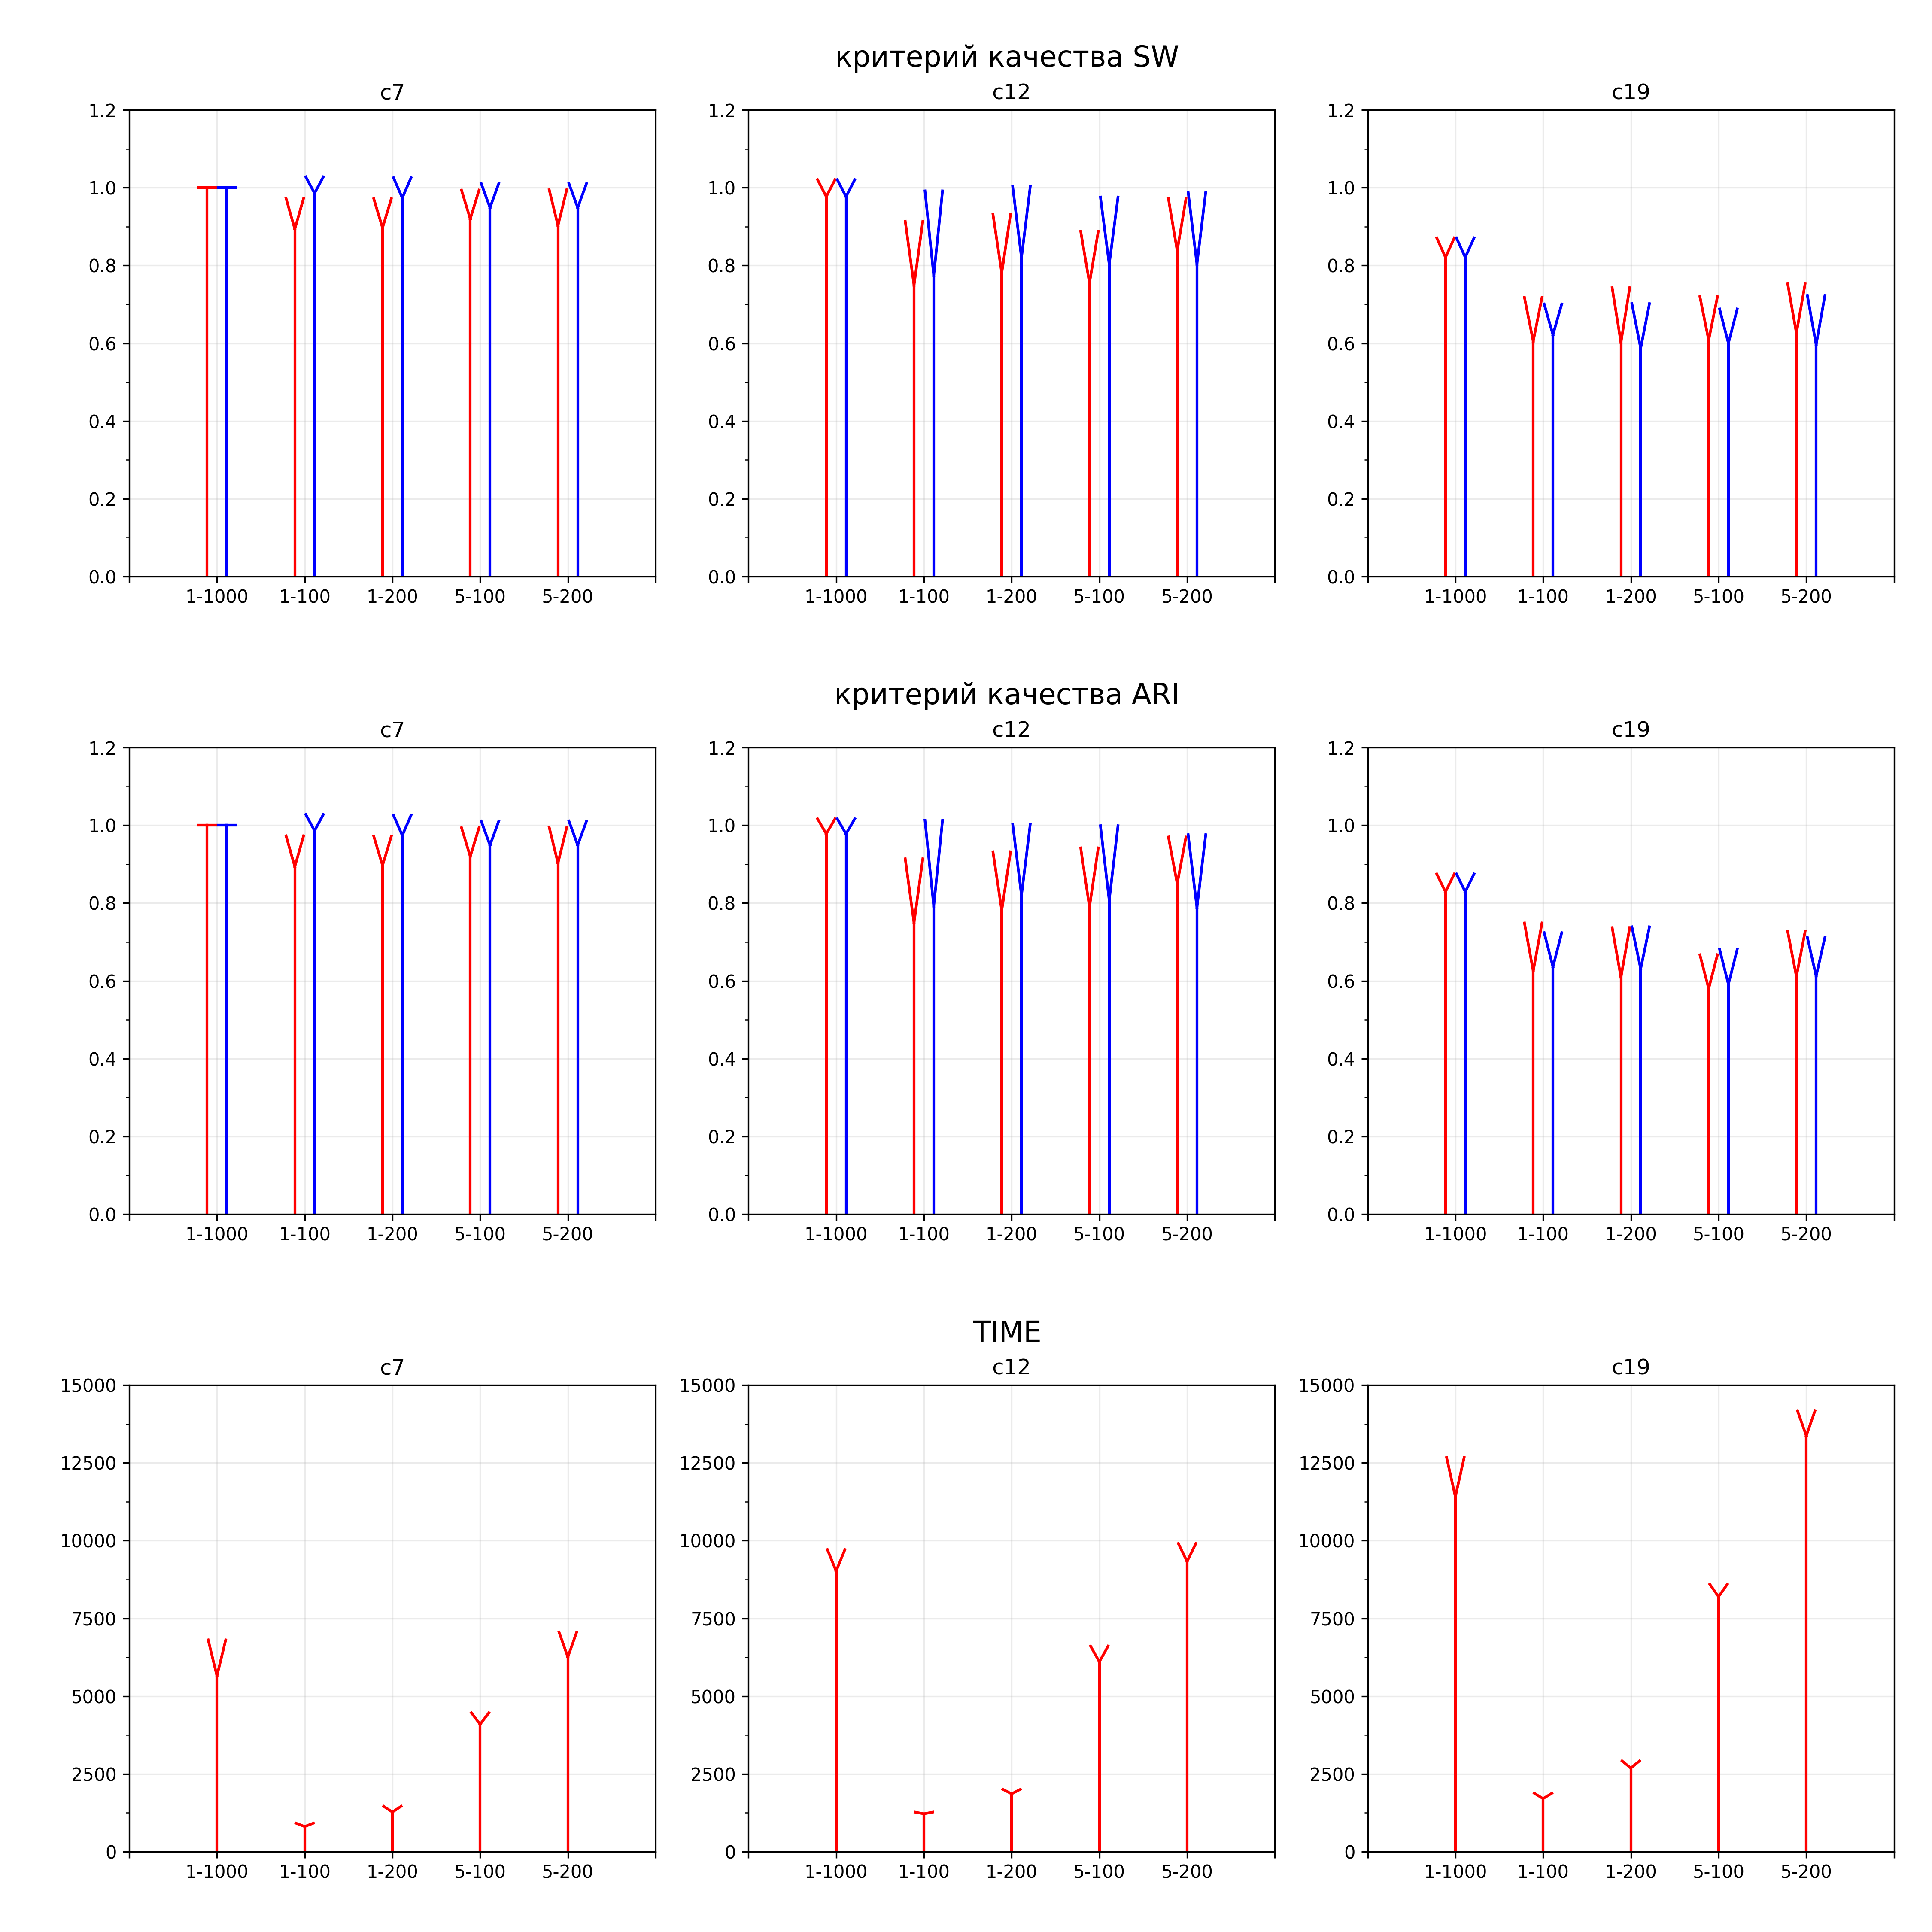
\includegraphics[width=\textwidth]{imgs/antennae.png} 
	\end{center}
	\caption{Диаграммы результатов}
	\label{fig:plots}
\end{figure}

Относительно сравнения используемых критериев качества можно сделать вывод, что характеристика SW показывает результаты, сопоставимые с результатами ARI. Наибольшее расхождение средних значений индекса ARI составило $ 0,044 $ для схемы перехода к подвыборкам 1-200 при 19 кластерах и втором подходе разрешения неопределённости. Таким образом, при выборе параметров \mbox{A-Ward$ _{p\beta} $} на реальных данных, для которых не известно истинное разбиение, применение характеристики SW оправдано.

При сравнении двух подходов разрешения неопределённости выясняется, что второй подход проявляет себя лучше, в среднем на $ 0,020 $ единиц ARI. Исходя из этого, второй подход разрешения неопределённости можно рекомендовать для практического применения.

Существенна экономия времени наблюдается только для однократного формирования выборки по схемам 1-100 и 1-200. Пятикратное формирование не даёт значимого ускорения и в некоторых случаях работает медленнее, чем полная схема 1-1000. В целом,  предлагаемое решение является эффективным лишь для небольшого числа кластеров и существенно ухудшает результат относительно анализа по полной выборке в противном случае. Любопытно также отметить, что значение индекса ARI разбиения, полученного по полной выборке 1-1000 для данных с семью кластерами, равно единице для всех 10 экспериментов, что вновь характеризует алгоритм \mbox{A-Ward$ _{p\beta} $} с лучшей стороны.

\section{Заключение}

Экспериментально проверено предположение о возможности перехода к подвыборкам при определении эффективных параметров алгоритма \mbox{A-Ward$ _{p\beta} $}. В эксперименте использованы синтетические данные для трёх случаев числа кластеров: 7, 12 и 19. Стоит отметить, что эти случаи соответствуют трём типам отношения числа кластеров и признаков: число кластеров меньше числа признаков, примерно равно и больше. Для алгоритмов, в которых используется аномальный кластер-анализ, рассмотрение указанных характерных случаев необходимо для разносторонней оценки их возможностей. При выборе наилучшей пары параметров из 1681 комбинаций были проанализированы два подхода разрешения неопределённости относительно нескольких максимумов характеристики качества. Для оценки правомерности выбора параметров по характеристике SW было произведено сравнение качества результирующего разбиения со случаем использования индекса ARI. Рассмотрено четыре схемы формирования подвыборок с однократным и пятикратным выбором по 100 и 200 объектов.

В ходе эксперимента в очередной раз была подтверждена эффективность \mbox{A-Ward$ _{p\beta} $}, что делает его привлекательным для дальнейших исследований, тем более что однозначного и полного ответа относительно быстрого выбора параметров $ p $ и $ \beta $ по результатам проведённой работы выработать не удалось. Для более разносторонней проработки темы следует провести аналогичные исследования для различных вариантов размерности данных и степени взаимного смешивания кластеров. Тем не менее, были получены следующие ценные выводы:

\begin{enumlist} 
	\item
	Применение эмпирической характеристики SW для выбора наилучшего разбиения оправдано;
	\item
	При решении практических задач, для выбора пары параметров из определённого множества возможных вариантов следует отдать предпочтение набору с наименьшим отклонением от усреднённых значений;
	\item
	Использование пятикраного формирования выборки теряет смысл ввиду больших временных затрат.
	\item
	Для случая с небольшим числом кластеров схема формирования выборки 1-100 может быть рекомендована как средство выбора рациональных параметров алгоритма и обеспечивает существенный выигрыш по времени.
\end{enumlist}

\begin{thebibliography}{10}


\bibitem{Mirkin-Vvedenie-v-analiz-dannyh}
{\it Миркин Б.Г.}
Введение в анализ данных. М.: Юрайт, 2015.

\bibitem{K-Means-canonical}
{\it Ball G.H., Hall D.J.}
A clustering technique for summarizing multivariate data, Behavioral Science. 1967. V. 12. Iss. 2. P. 153--155.

\bibitem{Ward-canonical}
{\it Joe H., Ward Jr.}
Hierarchical grouping to optimize an objective function, Journal of the American Statistical Association. 1963. V. 58. Iss. 301. P. 236--244.

\bibitem{Mirkin-Clustering-A-Data-Recovery-Approach}
{\it Mirkin B.}
Clustering: A Data Recovery Approach. London: CRC Press, 2012.

\bibitem{Anomalous-Clustring}
{\it Chiang M.M.-T., Mirkin B.}
Intelligent choice of the number of clusters in k-means clustering: an experimental study with different cluster spreads, Journal of Classification. 2010. V. 27. Iss. 1. P. 3--40.

\bibitem{Amorim-Makarenkov-Mirkin}
{\it de Amorim R.C., Makarenkov V., Mirkin B.}
\mbox{A-Ward$ _{p\beta} $}: Effective hierarchical clustering using the Minkowski metric and a fast \mbox{k-means} initialisation. Information Sciences. 2016. V. 370--371. P. 343--354.

\bibitem{SW-Based-Search}
{\it de Amorim R.C., Shestakov A., Mirkin B., Makarenkov V.}
The Minkowski central partition as a pointer to a suitable distance exponent and consensus partitioning. Pattern Recognition. 2017. V. 67. P. 62--72.

\bibitem{SW-Canonical}
{\it Rousseeuw P.}
Silhouettes: A graphical aid to the interpretation and validation of cluster analysis. Journal of Computational and Applied Mathematics. 1987. V.20. P. 53--65.

\bibitem{CrossValidation-canonical}
\textbf{Добавить какую-нибудь каноническую статью по кросс-валидации.}

\bibitem{Kovaleva}
{\it Kovaleva E., Mirkin B.}
Bisecting K-Means and 1D Projection Divisive Clustering: A Unified Framework and Experimental Comparison. Journal of Classification. 2015. V. 32. Iss. 3. P. 414--442.

\bibitem{ARI-canonical}
{\it Hubert L., Arabie P.}
Comparing partitions. Journal of Classification. 1985. V. 2. \mbox{Iss. 1.} P. 193--218.

\bibitem{SW1}
\textbf{Статья 1, в которой SW хорошо зарекомендовала себя}

\bibitem{SW2}
\textbf{Статья 2, в которой SW хорошо зарекомендовала себя}
\end{thebibliography}

\AdditionalInformation{Еремейкин П.А.}{Национальный исследовательский университет <<Высшая школа экономики>>, студент, Москва}{eremeykin@gmail.com}

\AdditionalInformation{Миркин Б.Г.}{Национальный исследовательский университет <<Высшая школа экономики>>, профессор, Москва}{bmirkin@hse.ru}



\end{document}
